\documentclass{article}
\usepackage{tikz}
\usepackage{pgfplots}
\usepackage{subcaption}

\begin{document}

\begin{figure}[hbt!]
    \centering
    \begin{subfigure}[t]{0.45\textwidth}
        \centering
        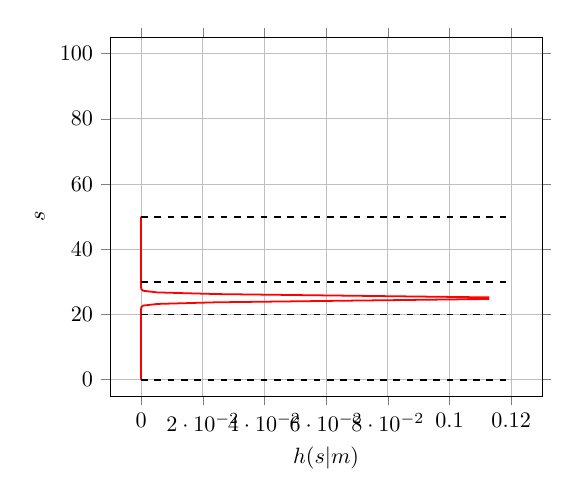
\begin{tikzpicture}[scale=0.8]
            \begin{axis}[
                grid=both,
                xlabel={$h(s|m)$},
                ylabel={$s$},
                ymin=-5, ymax=105,
                xmin=-0.01, xmax=0.13,
                tick align=outside
            ]
                \addplot[red, thick, domain=0:50, samples=100] (0.12*exp(-(x-25)*(x-25)),x);
                \addplot[color=black, thick, dashed] coordinates {(0, 0) (0.12, 0)};
                \addplot[color=black, thick, dashed] coordinates {(0, 20) (0.12, 20)};
                \addplot[color=black, thick, dashed] coordinates {(0, 30) (0.12, 30)};
                \addplot[color=black, thick, dashed] coordinates {(0, 50) (0.12, 50)};
            \end{axis}
        \end{tikzpicture}
        \caption{$h(s|m)$ при $m=50$}
        \label{fig:pic3}
    \end{subfigure}\hfill
    \begin{subfigure}[t]{0.45\textwidth}
        \centering
        \begin{tikzpicture}[scale=0.8]
            \begin{axis}[
                grid=both,
                xlabel={$m$},
                ylabel={$s$},
                xmin=-5, xmax=205,
                ymin=-5, ymax=105,
            ]
                % Main diagonal
                \addplot[red, domain=0:200, samples=100, dashdotted] {x/2};
                % Shaded region
                \addplot[name path=A, domain=10:200, samples=100, thick, dashed] {x/2 - 5};
                \addplot[name path=B, domain=0:190, samples=100, thick, dashed] {x/2 + 5};
    
                \addplot[name path=seg1, color=black, thick] coordinates {(0, 0) (100, 100)};
                \addplot[name path=seg2, color=black, thick] coordinates {(100, 100) (200, 100)};
                \addplot[name path=seg3, color=black, thick] coordinates {(200, 100) (100, 0)};
                \addplot[name path=seg4, color=black, thick] coordinates {(100, 0) (0, 0)};
                \addplot[red, opacity=0.3] fill between[of=seg1 and seg4];
                \addplot[red, opacity=0.3] fill between[of=seg2 and seg3];
    
                \addplot[red, opacity=0.3] fill between[of=A and B];
                \addplot[color=black, thick, dashed] coordinates {(0, 50) (50, 50)};
                \addplot[color=black, thick, dashed] coordinates {(0, 30) (50, 30)};
                \addplot[color=black, thick, dashed] coordinates {(0, 20) (50, 20)};
                \addplot[color=black, thick, dashed] coordinates {(0, 0) (50, 0)};
                \addplot[color=black, <->] coordinates {(50, 0) (50, 50)};
            \end{axis}
        \end{tikzpicture}
        \caption{$h(s|m)$ при $L=200, k=100$}
        \label{fig:pic4}
    \end{subfigure}
    \caption{Гипергеометрическое распределение $h(s|m)$}
\end{figure}

\end{document}
